\textbf{\textit{The Models}}---
As an example, we will consider the Majoron model. Nevertheless the study can also be applied to sterile neutrinos via magnetic portal, as we discuss in the Supplementary Materials. For the case of sterile neutrino with mixing portal, special care needs to be taken for resonant conversions in which case active neutrinos with plasma mass would travel as slowly as the sterile neutrinos at specific distances.
The relevant part of the Lagrangian in the Majoron case reads
\begin{align}
\mathcal{L} \supset -\frac{g_{\alpha\beta}}{2} \nu_\alpha \nu_\beta \phi - m_\phi \phi\phi^* + \text{h.c.}\,,
\end{align}
where $m_\phi$ is the Majoron mass and $g$ parametrizes interaction strength between $\phi$ and neutrinos. Consider flavor universal interaction, we abbreviate $g_{\alpha\beta}\equiv g$. Majorons are produced from neutrino coalescence in the star and then subsequently decay to a pair of neutrinos with the total decay width to all flavor of neutrinos given by $\Gamma_\phi = 3g^2 m_\phi/16 \pi$, and as a result, BSM neutrino flux is produced. 

Using data simulated by the Garching group for an $8.8 M_\odot$ progenitor star \cite{Huedepohl2010}, we obtained the fluxes of standard neutrino case that can be fitted to the parametrization in \cite{baxter2021snewpy} and the fluxes of Majoron $\phi$. Requiring the energy loss to Majorons to be less than 10\% of the standard neutrino energy, we can produce the cooling limit, which is in agreement with those obtained in literature \cite{Fiorillo:2022cdq}.
As mentioned above, for the regions below the coupling strength, Majorons produced will immediately stream out. Along its way towards the Earth, Majorons will decay to active neutrinos. For a given emission angle $\alpha$ of daughter neutrino relative to the direction of mother particle, and the angle $\theta$ at which the daughter neutrino arrives at the Earth, the time delay $\Delta t$, the arrival time of the daughter $\nu$ relative to that of the neutrinos produced in the explosion via SM processes, is \cite{Jaeckel:2017tud}
\begin{align}
    \Delta t = L_1/\beta + D_{\rm SN} \cos\theta-L_1 \cos\alpha -D_{\rm SN}\,,
    \label{eq:deltat}
\end{align}
with $D_{\rm SN}$ the distance between the SN and the Earth, $L_1$ the distance mother particles propagated before decaying, and $\beta$ being the speed of $\phi$. The flux of daughter $\nu$ is obtained by considering decays that only occur at $R^{\nu}_{\rm SN}\leq L_1 \leq L^{\rm max}_1$. As the smallest decay distance beyond which the daughter neutrino can escape the explosion unperturbed, we take $R^{\nu}_{\rm SN} = \unit[30]{km}$.
$L^{\rm max}_1$ corresponds to the distance $L_1$ with the largest time delay $\delta t$ \cite{Brdar:2023tmi}. 

\begin{figure}[t!]
    \centering
    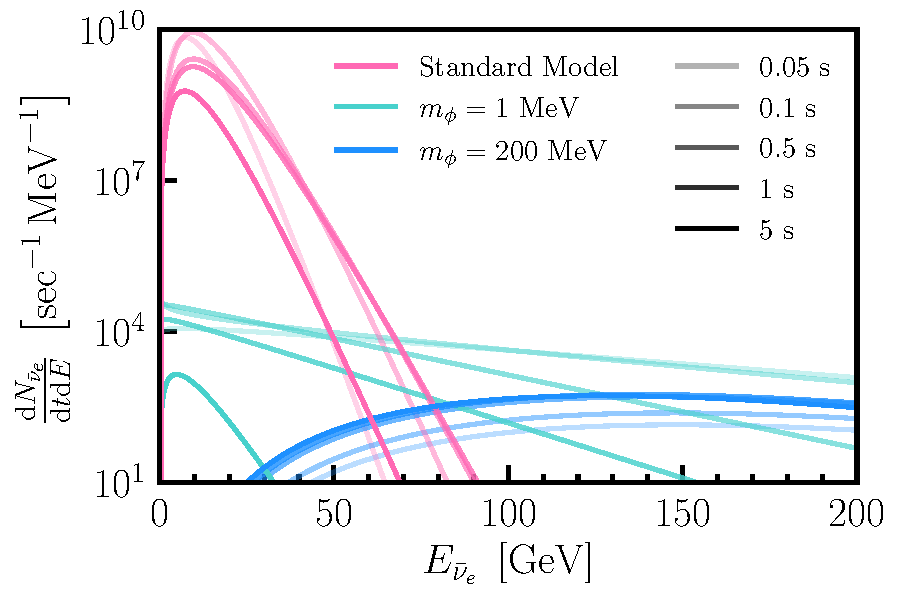
\includegraphics[width=0.47\textwidth]{figures/majoran_fluxes.pdf}
    \caption{\textit{\textbf{Flux of $\bar{\nu}_{e}$ from Standard Model production and two majoron hypotheses}}.
    We choose the parameters $g_\phi = 10^{-10.2}$ and $g_\phi = 10^{-11.8}$ for $m_\phi = \unit[1]{MeV}$ and $m_\phi = \unit[200]{MeV}$, respectively.
    In the case of the lower-mass model, the majoron can still travel relativistically, leading to a peak in the spectrum at an earlier time.
    In the case of the higher-mass model, the majoron travels subliminally, and thus, the flux peaks at later times.
    Since the dominant interaction is inverse beta decay at these energies, we expect the observed timing distribution to follow the $\bar{\nu}_{e}$
    }
    \label{fig:fluxes}
\end{figure}

For $D_{\rm SN} = \unit[10]{kpc}$ and $\delta t = \unit[100]{s}$ while larger values of $\delta t$ do not affect the limits obtained, we show in \cref{fig:fluxes} the differential fluxes of daughter neutrinos at different time for two benchmarks of the Majoron case, in comparison to the standard neutrino flux.
We can observe that the energy of neutrinos from Majoron decay extends to $\unit[100]{MeV}$ and above, as expected. For heavy Majoron case, the resulting neutrino flux typically is larger at later time, manifesting the time delay from slowly moving Majorons. 
The flux for light Majoron case contain very rich physics. Majorons, generating neutrinos with $E_\nu \geq \unit[150]{MeV}$, are nearly-relativistic with its daughter particles moving in parallel. In such a case, for couplings comparable to or larger than the one shown in \cref{fig:fluxes}, $\Delta t \sim L_d (1/\beta -1)\lesssim \unit[0.01]{sec}$, with $L_d = E_\phi/m_\phi \Gamma^{-1}_\phi \beta$ being the decay length of $\phi$ for the given $\phi$ energy $E_\phi$. The time dependence of neutrino flux thus are mainly inherited from the Majorons upon production, which exhibits in \cref{fig:fluxes} larger fluxes from producing Majorons from the denser and hotter core of SN at earlier time.
For neutrinos with lower energy, i.e $E_\nu \lesssim \unit[40]{MeV}$, the mother Majorons can be non-relativistic, resulting in $\Delta t \gtrsim \unit[0.04]{sec}$. This non-negligible time delay would shift the neutrino flux to later time, lowering the fluxes at earlier time as shown in \cref{fig:fluxes}. For the heavy mass benchmark in \cref{fig:fluxes}, we have $\Delta t \gtrsim \unit[10]{sec}$, which would yield the active neutrino flux at sizeable $t$.

%in details in the following, we consider energy deposits at the photomultipliers, 
%due to denser and hotter core of SN  as Majorans shortly after the bouncing time $t_{\rm bounce}$ from the hot dense core of SN. 

% \begin{figure*}
%     \centering
%     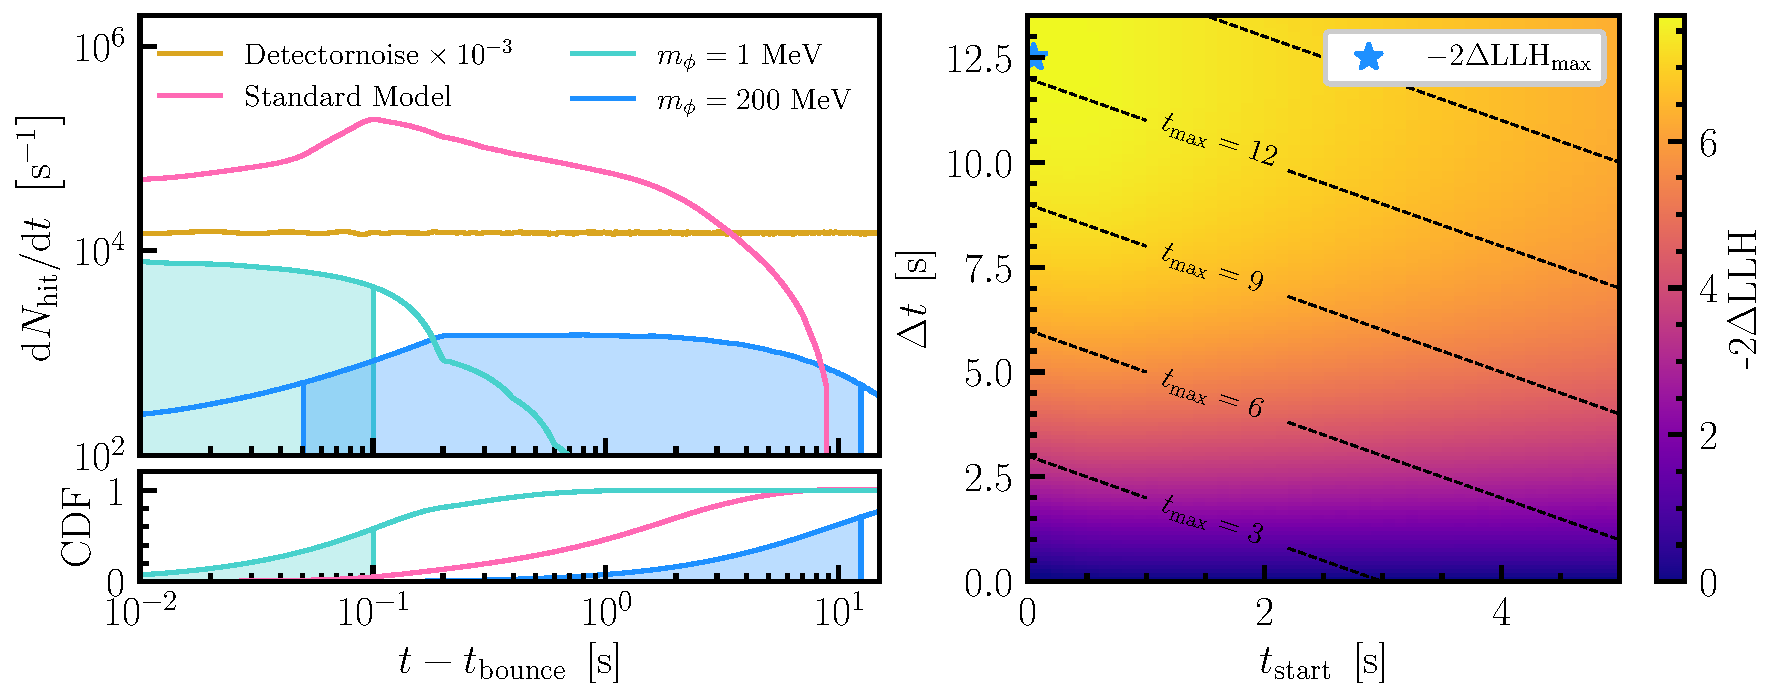
\includegraphics[width=0.95\textwidth]{figures/hits_and_likelihood.pdf}
%     \caption{\textbf{\textit{Timing profile of hits and test statistic as a function of the timing window.}}
%     These are the same points in the parameter space as Fig.~\ref{fig:fluxes}.
%     }
%     \label{fig:hits_and_likelihood}
% \end{figure*}
